\chapter{基于深度学习的目标检测技术}

\section{目标检测研究进展}
目标检测是计算机视觉领域重要的研究方向,有着长达20年的研究进程。目标检测任务通常被描述为:给定一张图像或者视频桢,定位其中所有感兴趣的目标,并确定每个目标的具体类别。图像中的目标可能出现在任何位置,目标的尺度和形态也存在各种各样的变化,图像的背景更是千差万别,这些因素导致目标检测并不是一个容易解决的问题。

目标检测第一个比较成功的案例,就是在大概2000年前后出现的Viola-Jones人脸检测器 \cite{viola-jones} \cite{via-jones-face}。这个方法的基本思路就是滑动窗口式的,用一个固定大小的窗口在输入图像上滑动,将窗口选定的图像区域送入分类器判断是人脸还是非人脸。滑动窗口的大小是固定,但是人脸的大小则各种各样,为了检测不同大小的人脸,还需要将输入图像缩放到不同大小,使得各种大小的人脸都能够在某个尺度上与窗口大小匹配。这种滑动窗口式的方法存在一个明显的问题,就是有太多的候选窗口去判断是人脸还是非人脸。为了加速这一过程,Viola-Jones检测器采用了级联的AdaBoost分类器,这种级联的结构能够逐级地过滤掉大量的非人脸窗口。值得一提的是,Viola-Jones人脸检测器之后被广泛应用在大量的电子产品中,例如数码相机中的人脸对焦功能,照相的时候,相机会自动检测人脸,然后根据人脸的位置把焦距调整得更好。

2005年出现的HOG特征描述子 \cite{hog} 是目标检测领域另一个里程碑式的进步。HOG是Histograms of Oriented Gradients的缩写,最早被应用在行人检测任务中。它的基本思想就是通过梯度或边缘的方向密度分布来表征一个对象,这种特征对于轮廓明显的对象具有较好的描述能力。HOG特征结合SVM分类器在行人检测领域大获成功,之后虽然有很多行人检测算法不断提出,但大多都是以HOG+SVM为基本框架。HOG特征对图像的几何和光学变化都能保持很好的不变性,不仅可以用来检测行人,也可以用来检测猫、狗等几乎任何物体。HOG的出现使得Viola-Jones检测器不再是目标检测的唯一选择。

继Viola-Jones检测器和HOG特征描述子之后,在2009年了出现了另外一个比较重要的方法:可变形部件模型 (Deformable Part Model,DPM)\cite{dpm}。目标大体上可以分为两类,刚性物体和非刚性物体。刚性物体,例如人脸,通常情况下不会有非常大的形变,比如嘴巴变到鼻子的上面,这类目标通常比较容易解决。非刚性物体,例如人体,可以看作一系列非刚性部件的铰接组合。DPM通过对部件进行建模可以很好地处理这种非刚性物体,它同时基于局部的部件和整体去做分类,在行人和车等任务上取得了较大的突破。DPM引入了对部件的建模,本身是一个很好的方法,但是被深度学习的光芒给盖过去了。深度学习对目标检测的精度带来了巨大的提升,所以研究DPM的一些学者也快速转移到深度学习上去了。

\begin{figure}[!t]
	\centering
	\includegraphics[scale=0.7]{detection_flow}
	\caption{传统目标检测算法的一般流程。}
	\label{detection_flow}
\end{figure}

总结下来,如图 \ref{detection_flow} 所示,传统的目标检测方法一般分为三个阶段:首先在给定图像上选择一些候选区域,然后对这些候选区域对应的图像块提取特征,最后使用预先训练好的分类器进行分类。
\begin{enumerate}
	\item 候选区域选择。\\
	由于目标可能出现在图像的任何位置,而且目标的尺度和长宽比也不确定,所以传统方法大多采用滑动窗口的机制对整幅图像进行遍历,而且需要设置不同的窗口大小和长宽比进行多次遍历。这种穷举的策略虽然包含了目标可能出现的所有位置,但是时间复杂度太高,而且冗余窗口太多容易增加``虚警率''。
	\item 候选区域特征提取。\\
	特征提取的好坏直接影响到分类的准确性,设计一个鲁棒的特征是研究人员坚持不懈的追求。然而,由于目标形态的多样性,图像背景的差异性等因素,研究人员手工设计的特征大多适用于特定目标种类,例如Haar \cite{via-jones-face},LBP \cite{lbp} 特征适用于人脸检测,HOG特征则对行人检测表现良好。
	\item 候选区域分类。\\
	分类器将候选区域判别为背景或者某个具体类别。目标检测任务中常用的分类器有SVM,AdaBoost等。
\end{enumerate}
传统目标检测算法主要存在两个问题:一个是基于滑动窗口的机制没有针对性,时间复杂度高,窗口冗余;二是手工设计的特征对于目标和背景的多样性变化不具备很好的鲁棒性。

\section{基于Region Proposal的深度学习目标检测算法}
对于传统目标检测算法中存在的两个问题,基于Region Proposal的深度学习目标算法给出了解决方案。

针对滑动窗口存在的问题,region proposal提供了解决办法。Region proposal(候选区域)就是图像中可能存在目标的位置。利用纹理、边缘、颜色等底层图像信息,region proposal提取算法能够保证在选取较少窗口(几千个甚至几百个)的情况下保持较高的目标召回率。这大大降低了后续计算的复杂度,并且获取的候选窗口甚至比滑动窗口的质量更高(滑动窗口通常以一定歩幅滑动)。比较常用的region proposal提取算法有selective search \cite{selective-search},edge box \cite{edge-box}和MCG \cite{mcg}。

有了候选区域,剩下的工作就是对候选区域对应的图像块进行分类。对于图像分类任务,深度卷积神经网络(Deep Convolutional Neural Network, DCNN)取得了巨大的突破。在2012年的ImageNet大规模视觉识别挑战赛(ILSVRC)上,Krizhevsky使用深度卷积神经网络AlexNet \cite{alexnet}将图片分类任务的top5-error降低到了15.3\%,而使用传统方法的第二名top5-error高达26.2\%。最新的神经网络,如ResNet \cite{resnet},Inception V4 \cite{inception-v4}等,已经将top5-error降到了4\%以内。2014年Ross B. Girshick等使用region proposal和DCNN代替传统方法使用的滑动窗口和手工设计特征,设计了R-CNN \cite{rcnn}目标检测框架,将PASCAL VOC 2010 \cite{pascal-voc-2010} 目标检测任务的state of the art由35.1\%提升到53.7\%,使得目标检测取得了巨大突破。

本节首先简要介绍一下深度卷积神经网络,然后介绍R-CNN目标检测框架及其加速改进版本SPP-net,Fast R-CNN,Faster R-CNN,并分析现有算法的不足,然后在下一节介绍本文提出的目标检测算法。

\subsection{深度卷积神经网络}
如图 \ref{cnn} 所示,一个简单的卷积神经网络由各种不同的层按照顺序排列组成。卷积神经网络主要由四种类型的层构成:卷积层(CONV),RELU层,池化层(POOL)和全连接层(FC),其中全连接层和常规神经网络中的一样。通过将这些层叠加起来,就可以构成一个完整的卷积神经网络。图 \ref{cnn} 中网络在CIFAR-10图像分类任务中的前向计算过程如下:
\begin{enumerate}
	\item 输入有RGB三个颜色通道的图像构成输入层,CIFAR-10中图像宽高均为32,即输入数据体的维度为$32\times32\times3$。
	\item 卷积层中每个神经元与输入层中的一个局部区域相连接,每个神经元计算与自己相连接的小区域与自己权重的内积。卷积层会计算所有神经元的输出,如果我们使用12个滤波器(也称作卷积核),得到的输出数据体的维度就是$32\times32\times12$。
	\item RELU层进行element-wise的激活函数操作,使用以零为阈值的$\max(0,x)$作为激活函数。该层对数据维度没有改变,输出数据体的维度还是$32\times32\times12$。
	\item
	池化层在空间维度(宽度和高度)上进行降采样(downsampling)操作,输出数据体的维度变为$16\times16\times12$。
	\item
	全连接层计算各个类别的评分,数据维度变为$1\times1\times10$,10路输出分别对应CIFAR-10中10个类别的评分值。全连接层与常规神经网络一样,每个神经元都与前一层中所有神经元相连接。
\end{enumerate}
\begin{figure}[!t]
	\centering
	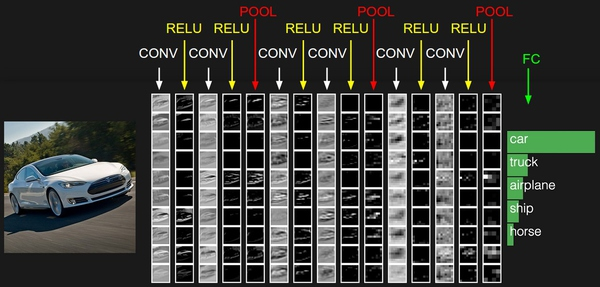
\includegraphics[width=\textwidth]{cnn}
	\caption{深度卷积神经网络在CIFAR-10 \cite{cifar-10} 图像分类任务上的应用示意图。注意:图中池化层的输出与输入具有相同的尺寸,这仅仅是为了示意,实际运行中池化层会进行降采样。输出层只显示了5个得分最高的评分值和对应的类别。}
	\label{cnn}
\end{figure}

\subsubsection{卷积层}
卷积层是卷积神经网络的核心层。